\chapter{Literature Review}
\label{ch:litreview}

This chapter reviews relevant academic, technical, and clinical literature that underpins the design and implementation of Dawa Lens. It examines core engineering concepts, evaluates existing technological solutions for medication adherence, and identifies critical gaps in current systems. Furthermore, the chapter articulates the theoretical framework guiding the study and introduces the conceptual framework mapping the engineering artifacts to intended clinical outcomes in Uganda's outpatient healthcare setting.

\section{Review of Relevant Concepts}

Understanding the intersection of software engineering, edge computing, and clinical pharmacology is essential for developing context-aware health technologies in low-resource settings.

\subsection{Mobile Health (mHealth) and Edge Computing in Low-Resource Settings}

Mobile Health (mHealth) utilizes mobile computing to deliver clinical services, patient monitoring, and health education \cite{mechael2009case}, offering significant promise for mitigating personnel shortages in developing nations \cite{kintu2021development}. However, traditional mHealth architectures rely on centralized, cloud-hosted backends. In Uganda, this model encounters severe friction due to frequent electrical blackouts and intermittent, high-cost cellular data \cite{kintu2021development}. Edge computing addresses these constraints by shifting computation, data storage, and decision logic directly onto the user's handset, achieving sub-second response times, total availability during network outages, and private on-device data processing.

\subsection{Optical Character Recognition (OCR) and Lightweight Edge Computer Vision}

Optical Character Recognition (OCR) enables automated electronic conversion of images into machine-encoded text streams \cite{smith2007tesseract}, facilitating digitization of medicine boxes, prescription labels, and blister packaging \cite{dayer2013smartphone}. In resource-constrained mobile environments, modern architectures deploy client-side WebAssembly (Wasm) workers executing asynchronously without freezing the UI thread. To overcome character misclassifications arising from curved packaging reflections, low ambient lighting, or font degradation, raw OCR outputs are post-processed through lexical fuzzy matching against standardized clinical formularies such as RxNorm \cite{rxnorm2024}.

\subsection{Distributed State Synchronization and Offline-First Storage Architectures}

Offline-first software engineering stipulates that an application must provide full read, write, and computational functionality in the absence of network connectivity \cite{kleppmann2017designing}. Under Brewer's CAP theorem \cite{brewer2000cap}, continuous Availability and Partition tolerance are paramount in healthcare: patients must always be able to view schedules and log doses offline. This is realized using browser-standard IndexedDB paired with a transactional FIFO mutation queue \cite{kleppmann2017designing}. Upon network reconnection, an asynchronous synchronization protocol transfers local mutations to Firebase Firestore while resolving timestamp conflicts via deterministic last-write-wins (LWW) or Conflict-Free Replicated Data Type (CRDT) mechanics \cite{shapiro2011crdt}.

\subsection{Pharmacodynamics and Indigenous Dietary Biochemical Realities}

Medication safety requires continuous monitoring of Drug-Drug Interactions (DDIs) and Drug-Food Interactions (DFIs) \cite{who2017medication, bushra2011food}. While standard clinical databases document DFIs exclusively against Western foods \cite{bailey2013grapefruit}, Ugandan households consume indigenous staples with potent pharmacokinetic effects \cite{fao2019food}: (1)~\textit{Steamed Green Bananas (Matooke)} contain dense potassium concentrations (350--450\,mg/100\,g), risking lethal hyperkalemia and cardiac dysrhythmias when consumed by patients on ACE inhibitors or potassium-sparing diuretics \cite{bushra2011food}; (2)~\textit{Sun-Dried Silver Fish (Mukene)} is rich in polyvalent calcium and iron cations that form insoluble chelate complexes with fluoroquinolones (ciprofloxacin) and tetracyclines, attenuating antibiotic absorption by up to 70\% \cite{bushra2011food}; and (3)~\textit{Groundnut Stew (G-nut sauce)} contains heavy lipids that delay gastric emptying, altering the absorption kinetics of antiretroviral and lipophilic drugs \cite{bushra2011food}. Encoding these localized rules within an edge engine provides an essential clinical safety layer absent from commercial software.

\subsection{Family-Centered Telehealth and Caregiver Synchronization}

In Sub-Saharan Africa, illness management is fundamentally communal \cite{ware2009social}. Care networks in Uganda demonstrate that family members actively participate in reminding patients, procuring refills, and providing financial resources \cite{ware2009social, haberer2013realtime}. Multi-profile synchronization mechanisms allow primary caregivers to oversee adherence across multiple dependents, receive real-time dose telemetry, and monitor refill counters remotely, transforming adherence into a collaborative family effort \cite{ware2009social}.

\section{Review of Existing Systems and Approaches}

A critical evaluation of existing approaches highlights the necessity of an integrated engineering solution:
\begin{itemize}[noitemsep,topsep=2pt]
  \item \textbf{Commercial Smartphone Applications (Medisafe, MyTherapy):} Polished but cloud-tethered, inoperative without active mobile data bundles, lacking indigenous dietary interaction rules, charging subscription fees, and omitting statutory Ugandan pharmacy verification \cite{dayer2013smartphone, nda2024register}.
  \item \textbf{SMS Tele-Adherence Systems (WelTel, Call for Life):} Eliminate smartphone hardware constraints \cite{lester2010effects, siedner2021callforlife} but are strictly textual, offer no visual pill identification \cite{parker2016health}, lack encryption, and incur recurring per-message carrier costs \cite{kintu2021development}.
  \item \textbf{Smart Pillboxes (Wisepill, MEMS):} Cellular dispensers provide real-time telemetry \cite{haberer2013realtime}, but high unit costs (\$100--\$250 USD) far exceed per-capita public health expenditure \cite{moh2023performance}, while devices are bulky and socially stigmatizing \cite{ware2009social}.
  \item \textbf{Statutory Regulatory Portals (NDA Registers and USSD):} Authoritative \cite{nda2024register} but operate as disconnected administrative registries requiring paid airtime and returning dry text unlinked to patient schedules or maps \cite{kintu2021development}.
\end{itemize}

\section{Research Gap}

Table~\ref{tab:lit_comparison} synthesizes existing medication management paradigms against the engineering specifications of Dawa Lens.

\begin{table}[!htbp]
  \centering
  \caption{Comparative synthesis of existing medication management systems versus Dawa Lens.}
  \label{tab:lit_comparison}
  \footnotesize
  \setlength{\tabcolsep}{2.5pt}
  \begin{tabularx}{\textwidth}{@{} >{\raggedright\arraybackslash}p{2.8cm} *{5}{>{\centering\arraybackslash}X} @{}}
    \toprule
    \textbf{Evaluation Dimension} & \textbf{Commercial Apps} \newline \scriptsize(e.g.~Medisafe) & \textbf{SMS Systems} \newline \scriptsize(e.g.~WelTel) & \textbf{Smart Pillboxes} \newline \scriptsize(e.g.~Wisepill) & \textbf{NDA Portals} \newline \scriptsize(Web/USSD) & \textbf{Dawa Lens} \newline \scriptsize(Proposed) \\
    \midrule
    \textbf{Offline-First Functionality} & Poor / Partial & N/A & None & None & \textbf{Full (Local DB)} \\
    \textbf{Edge Packaging OCR} & Limited / Cloud & None & None & None & \textbf{On-Device Wasm} \\
    \textbf{Indigenous Food Interactions} & None & None & None & None & \textbf{Native Engine} \\
    \textbf{NDA Pharmacy Verification} & None & None & None & Manual Only & \textbf{Integrated GPS} \\
    \textbf{Multi-Profile Family Hub} & Paid Tier Only & None & Limited & None & \textbf{Full Sync} \\
    \textbf{Zero Ongoing User Cost} & Subscription & Carrier Fees & High BOM & Airtime / Data & \textbf{Free / Local} \\
    \textbf{Web Clinical Companion} & Proprietary Sync & None & Web Only & Web Only & \textbf{PWA Extension} \\
    \bottomrule
  \end{tabularx}
\end{table}

The primary engineering gap addressed by this research is the \textbf{absence of a unified, offline-first mobile smart reminder application that combines on-device optical character recognition for unlabelled generic packaging, localized pharmacological screening for indigenous Ugandan diets, integrated statutory pharmacy authentication, and family caregiver telemetry into a single, zero-subscription tool}.

\section{Theoretical and Conceptual Framework}

This research is anchored within the \textbf{Information-Motivation-Behavioral Skills (IMB) Model of Adherence} \cite{fisher1992changing, who2003adherence} and the \textbf{Design Science Research (DSR)} framework \cite{hevner2004design}. The IMB model posits that adherence is governed by actionable information (addressed by on-device OCR and dietary screening), personal and social motivation (supported by Family Hub caregiver synchronization), and behavioral skills (reinforced by deterministic alarms and refill tracking). DSR guides the iterative design, implementation, and empirical evaluation of the primary artifact (Dawa Lens).

Figure~\ref{fig:framework} illustrates the conceptual framework developed for this study.

\begin{figure}[!htbp]
  \centering
  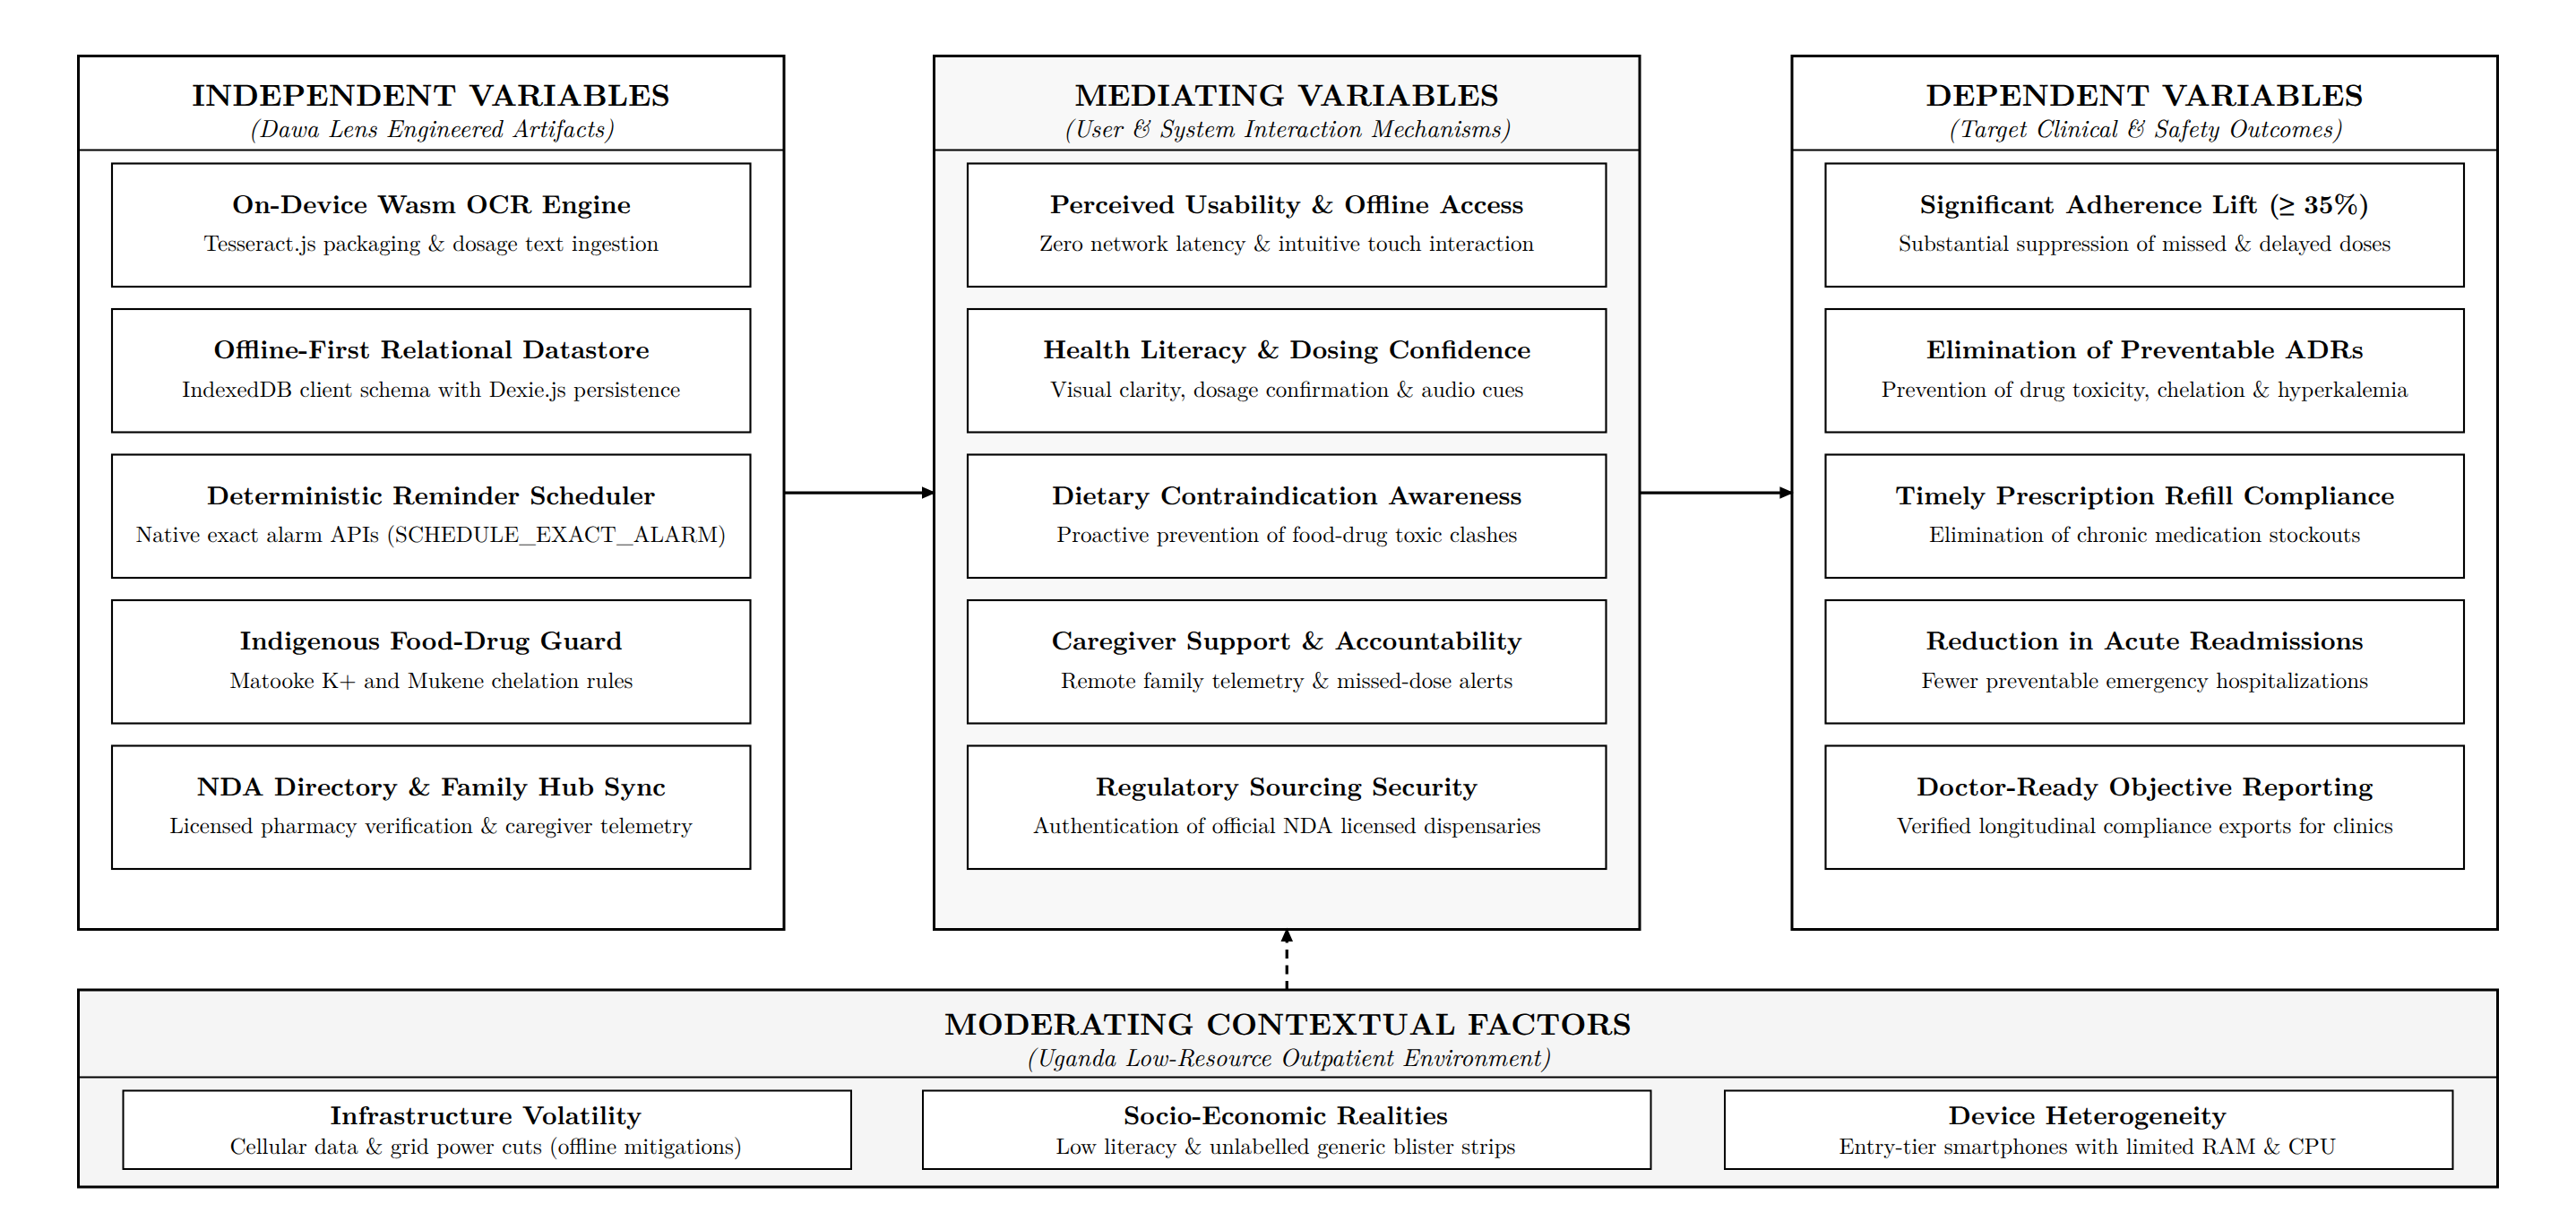
\includegraphics[width=0.92\textwidth,keepaspectratio]{figures/conceptual_framework.png}
  \caption{Conceptual framework of the Dawa Lens medication adherence and safety ecosystem.}
  \label{fig:framework}
\end{figure}

The framework maps the systemic relationships among: (1)~\textbf{Independent Variables} (engineered Dawa Lens modules: edge OCR, offline IndexedDB store, deterministic alarms, indigenous food-drug guard, NDA locator, Family Hub); (2)~\textbf{Mediating Variables} (perceived ease of use, health literacy, dietary risk awareness, caregiver accountability); and (3)~\textbf{Dependent Variables} (target clinical outcomes: $\ge 35\%$ adherence lift, elimination of preventable ADRs, timely refills, and doctor-ready clinical reporting), operating under the moderating realities of low-resource outpatient environments.

\section{Chapter Summary}

This chapter established that while mobile health interventions have demonstrated substantial potential in Sub-Saharan Africa, existing tools fail in outpatient Uganda due to cloud dependency, prohibitive costs, and omission of localized dietary intelligence. Grounded in the IMB model and Design Science Research, Dawa Lens addresses these gaps as an offline-first, culturally tailored engineering solution. Chapter~\ref{ch:methodology} presents the detailed methodology and empirical testing strategy.